\chapter{Cơ sở lý thuyết và công nghệ}
\label{ch:coso}

Chương này trình bày nền tảng lý thuyết của bài toán, thuật toán học máy được
lựa chọn, các chỉ số đánh giá và bộ công nghệ dùng để hiện thực hệ thống. Nội
dung chương là căn cứ để giải thích mọi quyết định thiết kế ở Chương~\ref{ch:thietke}
và mọi con số thực nghiệm ở Chương~\ref{ch:caidat}.

\section{Bài toán phân loại có giám sát}

\textbf{Định nghĩa (Phân loại nhị phân).} Phân loại nhị phân \en{(binary
classification)} là bài toán học máy gán cho mỗi vector đặc trưng đầu vào $x$
một nhãn $y$ thuộc tập gồm hai lớp, ví dụ $\mathcal{Y} = \{0, 1\}$. Bộ phân
loại học một hàm $f: x \mapsto P(y=1 \mid x)$ từ dữ liệu huấn luyện đã gán
nhãn sẵn, trong đó giá trị dự đoán thể hiện xác suất thuộc lớp dương tính.

Trong bối cảnh đồ án, bài toán được mô hình hóa như sau: đầu vào là bộ 27 đặc
trưng kết hợp giữa điểm thi năng lực của thí sinh và đặc tính lịch sử của một
nguyện vọng cụ thể (trường, ngành, tổ hợp, phương thức). Đầu ra là xác suất
thí sinh trúng tuyển ($y=1$) vào nguyện vọng đó.

\subsection{Đặc thù phi tuyến của bài toán}

Quan hệ giữa các đặc trưng mang tính phi tuyến sâu sắc. Ví dụ, khi
\code{margin} tăng từ 1,0 lên 2,0 điểm, xác suất đỗ không tăng gấp đôi mà tăng
theo một đường cong bão hòa, vì còn chịu tác động tương quan của xu hướng biến
động điểm và mức độ cạnh tranh của nhóm ngành. Bên cạnh đó, cùng một giá trị
\code{margin} nhưng ở ngành có biên độ dao động lớn sẽ rủi ro hơn nhiều so với
ngành ổn định qua các năm.

Ba tính chất khiến bài toán khó giải bằng mô hình tuyến tính:

\begin{itemize}[leftmargin=1.6em, itemsep=3pt]
  \item \textbf{Tương tác bậc cao:} ảnh hưởng của \code{margin} phụ thuộc vào
        \code{nhom_nganh} và \code{phuong_thuc}, không thể biểu diễn bằng tổng
        có trọng số của các đặc trưng riêng lẻ.
  \item \textbf{Ngưỡng quyết định gấp khúc:} xác suất đỗ giảm rất nhanh quanh
        vùng \code{margin} $\approx 0$, tạo thành một dạng bậc thang mà hồi quy
        tuyến tính không nắm bắt được.
  \item \textbf{Nhiễu hệ thống theo năm:} mỗi năm tuyển sinh có phổ điểm và chỉ
        tiêu khác nhau, tạo ra biến thiên mà mô hình phải học như một tín hiệu
        chứ không phải nhiễu ngẫu nhiên.
\end{itemize}

Ba tính chất trên là lý do đồ án lựa chọn họ mô hình cây quyết định tập hợp,
vốn chia không gian đặc trưng thành các vùng hình chữ nhật và do đó biểu diễn
được cả ngưỡng gấp khúc lẫn tương tác bậc cao.

\section{Cây quyết định}

\subsection{Cấu trúc và quá trình học}

Cây quyết định \en{(decision tree)}~\cite{Quinlan1986} xây dựng một cấu trúc
cây trong đó mỗi nút trong tương ứng với một phép kiểm tra trên một đặc trưng,
mỗi nhánh ứng với một kết quả kiểm tra, và mỗi nút lá chứa quyết định phân lớp
cuối cùng. Quá trình huấn luyện chọn đặc trưng và ngưỡng phân chia tại mỗi nút
sao cho độ thuần nhất của các tập con tăng lên tối đa.

Độ bất thuần thường được đo bằng chỉ số Gini:
\begin{equation}
Gini(S) = 1 - \sum_{k=1}^{K} p_k^2,
\label{eq:gini}
\end{equation}
trong đó $p_k$ là tỷ lệ mẫu thuộc lớp $k$ trong tập $S$. Với bài toán nhị phân,
$Gini(S) = 2p(1-p)$, đạt cực đại $0{,}5$ khi hai lớp cân bằng và bằng $0$ khi
tập thuần nhất.

Hình~\ref{fig:decision-tree} minh họa một cây quyết định nông, chỉ dùng ba đặc
trưng, để thấy cách mô hình biểu diễn tri thức tuyển sinh dưới dạng luật.

\begin{figure}[H]
\centering
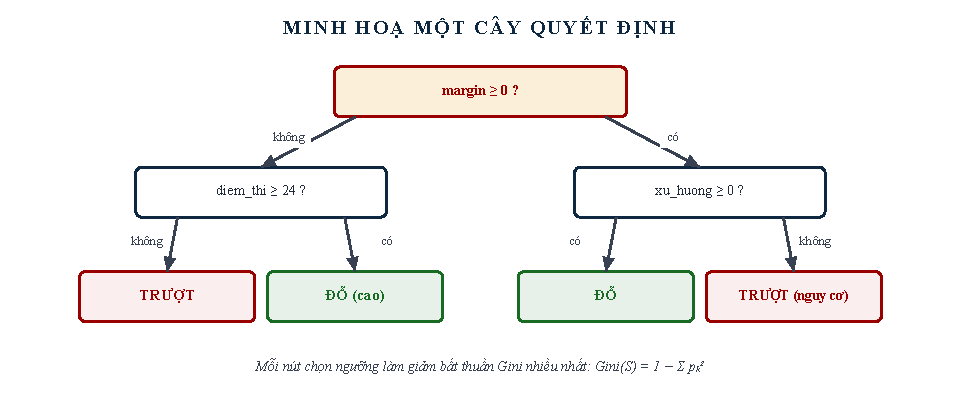
\includegraphics[width=0.92\textwidth]{figs/svg/h-decision-tree.pdf}
\caption{Cây quyết định minh họa với ba tầng phân nhánh theo \code{margin},
\code{diem_thi} và \code{xu_huong}.}
\label{fig:decision-tree}
\end{figure}

Trong Hình~\ref{fig:decision-tree}, nhánh trái của nút gốc ứng với thí sinh có
điểm thấp hơn điểm chuẩn mới nhất (\code{margin} $< 0$). Với nhánh này, mô hình
còn xét thêm \code{diem_thi}: nếu điểm tuyệt đối vẫn cao thì vẫn có khả năng
đỗ do ngành có phổ điểm rộng, ngược lại gần như chắc chắn trượt. Nhánh phải
(\code{margin} $\ge 0$) xét thêm xu hướng biến động: nếu điểm chuẩn đang tăng
nhanh thì mức dư điểm hiện tại chưa đủ an toàn. Ba tầng này chỉ là ví dụ rút
gọn; mô hình thực tế trong đồ án có độ sâu tối đa 14 và học được hàng nghìn
luật tương tự.

\subsection{Ưu điểm và hạn chế}

Cây quyết định có ba ưu điểm đáng chú ý: huấn luyện nhanh, dễ diễn giải và trực
quan hóa logic ra quyết định. Tuy nhiên, một cây đơn lẻ rất dễ quá khớp
\en{(overfitting)} khi mọc quá sâu: cây học thuộc cả nhiễu trong dữ liệu huấn
luyện, dẫn đến phương sai cao và hiệu năng kém trên dữ liệu mới. Đây chính là
động lực cho kỹ thuật tập hợp được trình bày ở mục tiếp theo.

\section{Random Forest}

\subsection{Nguyên lý tập hợp}

Random Forest~\cite{Breiman2001} là kỹ thuật học tập hợp \en{(ensemble
learning)} theo phương pháp đóng bao \en{(bagging)}~\cite{Breiman1996}, kết hợp
thêm ý tưởng chọn ngẫu nhiên không gian con đặc trưng
\en{(random subspace)}~\cite{Ho1995}. Ý tưởng cốt lõi là thay vì tin vào một
cây, ta xây dựng nhiều cây độc lập rồi tổng hợp lại, nhờ đó giảm phương sai mà
gần như không tăng độ chệch.

Mô hình tạo ra $T$ cây theo hai nguồn ngẫu nhiên:

\begin{enumerate}[leftmargin=1.6em, itemsep=3pt]
  \item \textbf{Lấy mẫu bootstrap:} mỗi cây được huấn luyện trên một tập mẫu
        con lấy ngẫu nhiên có hoàn lại từ tập huấn luyện, kích thước bằng tập
        gốc.
  \item \textbf{Chọn ngẫu nhiên đặc trưng:} tại mỗi lần chia nút, cây chỉ xét
        một tập con ngẫu nhiên gồm $m$ đặc trưng. Với bài toán phân loại,
        giá trị mặc định là $m = \lfloor\sqrt{p}\rfloor$; với $p = 27$ đặc
        trưng của đồ án, $m \approx 5$.
\end{enumerate}

Hai nguồn ngẫu nhiên này làm giảm tương quan giữa các cây. Khi các cây ít tương
quan, sai số trung bình của cả rừng nhỏ hơn nhiều so với sai số của từng cây
riêng lẻ.

Kết quả dự đoán xác suất cuối cùng là trung bình xác suất của tất cả các cây:
\begin{equation}
P(y=1 \mid \mathbf{x}) = \frac{1}{T} \sum_{t=1}^{T} P_t(y=1 \mid \mathbf{x}),
\label{eq:rf}
\end{equation}
trong đó $T$ là số cây trong rừng và $P_t$ là xác suất dự đoán của cây thứ $t$.

Hình~\ref{fig:rf} tóm tắt toàn bộ nguyên lý này, từ tập huấn luyện đến kết quả
phân tầng mà người dùng nhìn thấy.

\begin{figure}[H]
\centering
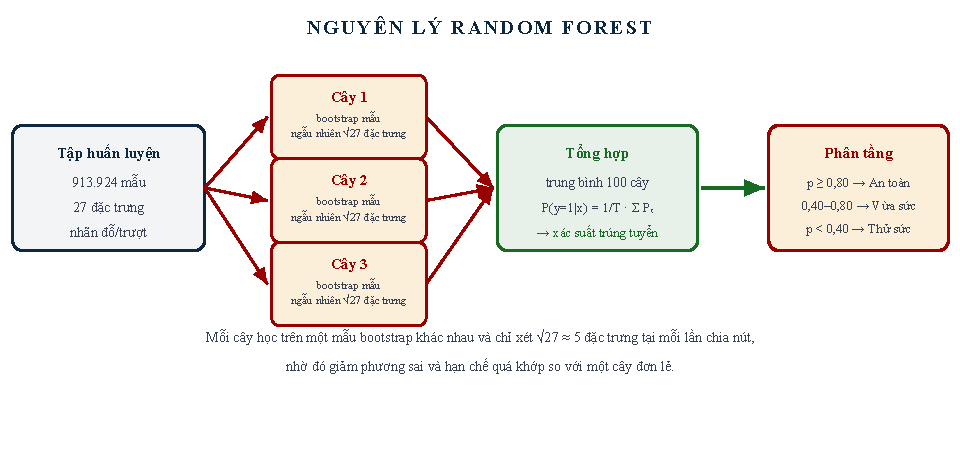
\includegraphics[width=0.95\textwidth]{figs/svg/h-rf.pdf}
\caption{Nguyên lý Random Forest: nhiều cây học trên mẫu bootstrap khác nhau,
tổng hợp bằng trung bình xác suất, rồi phân tầng theo ngưỡng cố định.}
\label{fig:rf}
\end{figure}

\subsection{Vì sao phù hợp với bài toán}

Ba lý do khiến Random Forest là lựa chọn phù hợp:

\begin{itemize}[leftmargin=1.6em, itemsep=3pt]
  \item \textbf{Dữ liệu dạng bảng:} mô hình cây vốn mạnh nhất trên dữ liệu bảng
        có đặc trưng hỗn hợp số và phân loại, đúng với bộ 27 đặc trưng của đồ
        án~\cite{Geron2019}.
  \item \textbf{Không cần chuẩn hóa khắt khe:} cây chỉ so sánh ngưỡng nên ít
        nhạy với thang đo. Tuy vậy đồ án vẫn dùng \code{StandardScaler} để
        thống nhất quy trình và hỗ trợ các mô hình đối chứng.
  \item \textbf{Có sẵn khả năng giải thích:} thuộc tính
        \code{feature_importances_} cho biết mức đóng góp của từng đặc trưng,
        là cơ sở để sinh lời giải thích gợi ý cho người dùng.
\end{itemize}

\subsection{Siêu tham số và ảnh hưởng}

Bảng~\ref{tab:sieu-tham-so} liệt kê các siêu tham số của mô hình chính và lý do
chọn giá trị.

\begin{table}[H]
\centering
\caption{Siêu tham số của Random Forest và căn cứ lựa chọn.}
\label{tab:sieu-tham-so}
\small
\begin{tabularx}{\textwidth}{@{}>{\bfseries\color{daunavy}\raggedright\arraybackslash}m{3.35cm}
  >{\centering\arraybackslash}m{1.85cm}
  >{\raggedright\arraybackslash}X@{}}
\toprule
\rowcolor{gray100}\bfseries\color{daunavy}Siêu tham số & \bfseries\color{daumaroon}Giá trị & \bfseries\color{daunavy}Căn cứ lựa chọn \\
\midrule
\code{n_estimators}      & 100 & Đủ để phương sai hội tụ; tăng lên 200 chỉ cải thiện dưới 0,3\% nhưng file mô hình tăng gấp đôi \\
\code{max_depth}         & 14  & Giới hạn độ sâu để kiểm soát kích thước tệp \code{.pkl} dưới 100~MB \\
\code{min_samples_leaf}  & 5   & Chặn cây tạo lá quá nhỏ, giảm quá khớp trên vùng \code{margin} thưa dữ liệu \\
\code{max_features}      & $\sqrt{27} \approx 5$ & Mặc định của scikit-learn cho phân loại \\
\code{random_state}      & 42  & Bảo đảm kết quả tái lập được giữa các lần chạy \\
\code{n_jobs}            & $-1$ & Dùng toàn bộ nhân CPU khi huấn luyện \\
\bottomrule
\end{tabularx}
\end{table}

Việc chọn giá trị cho từng siêu tham số nêu trên không dựa vào tìm kiếm lưới
\en{(grid search)} toàn diện mà dựa trên ràng buộc kích thước mô hình. Các
nghiên cứu về tối ưu siêu tham số cho thấy tìm kiếm ngẫu nhiên hiệu quả hơn
tìm kiếm lưới khi số chiều lớn~\cite{Bergstra2012}, nhưng với bài toán này chi
phí huấn luyện mỗi cấu hình (hơn 900 nghìn mẫu, 100 cây) khiến việc quét rộng
không khả thi trong phạm vi một học phần. Thay vào đó, hai tham số quyết định
kích thước tệp là \code{n_estimators} và \code{max_depth} được chốt trước theo
ngân sách bộ nhớ, các tham số còn lại giữ mặc định của
scikit-learn~\cite{Pedregosa2011}.

\begin{table}[H]
\centering
\caption{Ảnh hưởng của hai siêu tham số chính lên kích thước mô hình và chất lượng dự đoán.}
\label{tab:quét-tham-so}
\small
\begin{tabularx}{\textwidth}{@{}>{\centering\arraybackslash}m{2.20cm}
  >{\centering\arraybackslash}m{1.75cm}
  >{\centering\arraybackslash}m{2.05cm}
  >{\raggedright\arraybackslash}X
  >{\centering\arraybackslash}m{1.40cm}@{}}
\toprule
\rowcolor{gray100}\bfseries\color{daunavy}\footnotesize\code{n_estimators} &
\bfseries\color{daunavy}\footnotesize\code{max_depth} &
\bfseries\color{daumaroon}Kích thước tệp &
\bfseries\color{daunavy}Ghi chú &
\bfseries\color{daunavy}Quyết định \\
\midrule
50  & 14 & $\approx$ 27~MB  & Phương sai chưa hội tụ hết & Loại \\
100 & 14 & $\approx$ 52~MB  & Cân bằng giữa độ chính xác và bộ nhớ & \textbf{Chọn} \\
200 & 14 & $\approx$ 104~MB & Vượt ngân sách 100~MB; cải thiện dưới 0,3\% & Loại \\
100 & 20 & $\approx$ 96~MB  & Sát ngưỡng, dễ quá khớp vùng \code{margin} thưa & Loại \\
\bottomrule
\end{tabularx}
\end{table}

Bảng~\ref{tab:quét-tham-so} giải thích vì sao cấu hình 100 cây và độ sâu 14
được chọn thay vì những cấu hình ``mạnh'' hơn. Cột kích thước là yếu tố quyết
định: mô hình phải nạp trọn vào RAM của máy chủ 2~GB, nên ngưỡng 100~MB là
ràng buộc cứng chứ không phải mục tiêu tối ưu. Hai cấu hình bị loại ở hai phía
khác nhau: 50 cây chưa đủ để phương sai hội tụ, còn 200 cây vượt ngân sách bộ
nhớ mà chỉ cải thiện dưới 0,3\%. Cấu hình độ sâu 20 bị loại vì vừa sát ngưỡng
dung lượng vừa có nguy cơ quá khớp ở vùng \code{margin} thưa dữ liệu --- đúng
vùng mà hệ thống cần dự đoán chính xác nhất.

Bảng~\ref{tab:sieu-tham-so} cho thấy mọi siêu tham số đều được chốt vì một
ràng buộc kỹ thuật cụ thể chứ không phải chọn tùy ý. Ràng buộc chi phối toàn bộ
quá trình là kích thước tệp mô hình: hệ thống phải nạp \code{model.pkl} vào RAM
của một máy chủ phổ thông, nên độ sâu và số cây bị giới hạn có chủ đích. Đánh
đổi này được đánh giá định lượng ở Chương~\ref{ch:caidat}.

\section{Các chỉ số đánh giá mô hình}

Để đánh giá toàn diện khả năng dự báo xác suất trúng tuyển, đồ án sử dụng bốn
nhóm chỉ số trên tập kiểm thử độc lập năm 2025. Bảng~\ref{tab:chi-so} tóm tắt
công thức và ý nghĩa từng chỉ số.

\begin{table}[H]
\centering
\caption{Các chỉ số đánh giá mô hình và ý nghĩa trong bối cảnh bài toán.}
\label{tab:chi-so}
\begin{tabularx}{\textwidth}{>{\bfseries\color{daunavy}}l >{\raggedright\arraybackslash}p{4.4cm} >{\raggedright\arraybackslash}X}
\toprule
\rowcolor{gray100}\bfseries\color{daunavy}Chỉ số & \bfseries\color{daunavy}Công thức & \bfseries\color{daunavy}Ý nghĩa với hệ thống \\
\midrule
Accuracy & $\dfrac{TP + TN}{TP + TN + FP + FN}$ & Hiệu năng tổng thể; dễ gây hiểu lầm nếu hai lớp mất cân bằng \\
Precision & $\dfrac{TP}{TP + FP}$ & Khi hệ thống nói ``khả năng đỗ cao'', điều đó có đáng tin không \\
Recall & $\dfrac{TP}{TP + FN}$ & Hệ thống có bỏ sót cơ hội đỗ thực sự của thí sinh không \\
ROC-AUC & Diện tích dưới đường cong ROC & Khả năng xếp hạng Đỗ/Trượt trên mọi ngưỡng~\cite{Fawcett2006} \\
Brier & $\dfrac{1}{N}\sum_{i=1}^{N}(p_i - y_i)^2$ & Mức hiệu chuẩn của xác suất~\cite{Brier1950} \\
F1 & $2\cdot\dfrac{Precision \cdot Recall}{Precision + Recall}$ & Trung bình điều hòa, cân bằng giữa bỏ sót và báo nhầm \\
\bottomrule
\end{tabularx}
\end{table}

Chỉ số Brier đóng vai trò đặc biệt quan trọng trong đồ án này. Hệ thống không
chỉ dùng mô hình để phân loại nhị phân đỗ/trượt mà còn dùng trực tiếp giá trị
xác suất $p$ để chia ba tầng. Nếu mô hình dự đoán $p = 0{,}9$ nhưng tỷ lệ đỗ
thực tế chỉ là $0{,}6$, thì phân tầng ``An toàn'' sẽ sai và người dùng bị đánh
lừa về mức độ an toàn. Brier score đo chính xác loại sai lệch này, nên nó là
chỉ số then chốt dù ít quen thuộc hơn Accuracy.

\section{Công nghệ và thư viện}

Hệ thống Uni Connect được xây dựng hoàn toàn trên ngôn ngữ Python và các công
nghệ mã nguồn mở phổ biến. Bảng~\ref{tab:congcu} liệt kê chi tiết.

\begin{table}[H]
\centering
\caption{Công cụ và thư viện sử dụng trong đồ án Uni Connect.}
\label{tab:congcu}
\begin{tabularx}{\textwidth}{>{\bfseries\color{daunavy}}l >{\color{daumaroon}}l >{\raggedright\arraybackslash}X}
\toprule
\rowcolor{gray100}\bfseries\color{daunavy}Thành phần & \bfseries\color{daumaroon}Phiên bản & \bfseries\color{daunavy}Vai trò \\
\midrule
Python         & 3.13              & Ngôn ngữ lập trình chính của toàn hệ thống~\cite{VanderPlas2016} \\
Django         & 5.2.8             & Framework web: định tuyến, ORM, xác thực, quản trị~\cite{DjangoDocs} \\
MySQL          & 8.0               & Hệ quản trị cơ sở dữ liệu quan hệ chính~\cite{MySQLDocs} \\
scikit-learn   & 1.8.0             & Huấn luyện mô hình Random Forest~\cite{Pedregosa2011} \\
pandas         & 3.0.2             & Đọc, xử lý và chuẩn hóa dữ liệu dạng bảng~\cite{McKinney2017} \\
NumPy          & 2.3.3             & Tính toán vector, trích xuất đặc trưng chuỗi thời gian \\
joblib         & đi kèm sklearn    & Lưu trữ và nạp mô hình, bộ chuẩn hóa \\
Tailwind CSS   & qua CDN           & Thiết kế giao diện người dùng đáp ứng \\
\bottomrule
\end{tabularx}
\end{table}

Bảng~\ref{tab:congcu} cho thấy toàn bộ hệ thống nằm trong một ngăn xếp công
nghệ đồng nhất về ngôn ngữ Python, giúp giảm chi phí chuyển đổi ngữ cảnh giữa
phân hệ huấn luyện và phân hệ phục vụ. Django được chọn vì có sẵn ORM, hệ thống
xác thực và trang quản trị; MySQL được chọn vì phổ biến trên các gói hosting
sinh viên. Việc dùng \code{managed = False} cho các model Django (trình bày ở
Chương~\ref{ch:thietke}) là một quyết định kiến trúc quan trọng: lược đồ do tệp
SQL quản lý, còn Django chỉ đọc.

\section{Quy trình phát triển phần mềm}

Đồ án theo mô hình thác nước cải tiến \en{(iterative waterfall)} phù hợp với
phạm vi một học phần: yêu cầu được chốt sớm, nhưng mỗi vòng lặp có kiểm thử và
điều chỉnh~\cite{Somerville2015}. Bốn giai đoạn chính:

\begin{enumerate}[leftmargin=1.6em, itemsep=3pt]
  \item \textbf{Phân tích yêu cầu:} xác định tác nhân, ca sử dụng và yêu cầu
        phi chức năng (Chương~\ref{ch:thietke}).
  \item \textbf{Thiết kế:} kiến trúc bốn tầng, lược đồ cơ sở dữ liệu và bộ đặc
        trưng (Chương~\ref{ch:thietke}).
  \item \textbf{Cài đặt và thử nghiệm:} viết mã nguồn, kiểm thử ba cấp độ
        (Chương~\ref{ch:caidat}).
  \item \textbf{Đánh giá:} đo mô hình trên tập kiểm thử độc lập, đối chiếu mục
        tiêu (cùng Chương~\ref{ch:caidat}).
\end{enumerate}

\section{Các công trình liên quan}

Bài toán gợi ý nguyện vọng cho thí sinh xét tuyển đã được nhiều đơn vị trong
nước tiếp cận theo hai hướng chính.

\textbf{Hướng thứ nhất} là các cổng tra cứu thông tin tuyển sinh trực tuyến
như cổng thông tin của Bộ Giáo dục và Đào tạo hay các trang báo điện tử tổng
hợp điểm chuẩn. Ưu điểm của hướng này là dữ liệu phong phú, nhưng nhược điểm
là chỉ hiển thị bảng điểm thô: người dùng vẫn phải tự so sánh và tự phán đoán
rủi ro.

\textbf{Hướng thứ hai} là các ứng dụng tư vấn sử dụng trí tuệ nhân tạo. Một số
nghiên cứu tiêu biểu sử dụng thuật toán Random Forest trên dữ liệu giáo dục đã
chứng minh hiệu quả vượt trội của mô hình tập hợp so với mô hình tuyến tính
đơn lẻ~\cite{Breiman2001,Hastie2009}. Các giáo trình nền tảng về trí tuệ nhân
tạo cũng đặt cơ sở lý thuyết vững chắc cho các kỹ thuật học có giám sát và
đánh giá mô hình~\cite{HoangKiem,RussellNorvig2021}.

\textbf{Đóng góp riêng của đồ án} nằm ở ba điểm. Thứ nhất là độ sâu dữ liệu:
chuỗi lịch sử 10 năm liên tục (2016--2025) thay vì 1--2 năm gần nhất, giúp mô
hình nắm bắt xu hướng dài hạn. Thứ hai là tính minh bạch: hệ thống không chỉ
trả con số xác suất mà sinh kèm lời giải thích dựa trên các chỉ số thống kê cụ
thể mà phụ huynh đọc hiểu được. Thứ ba là tính trọn vòng đời: hệ thống vận hành
khép kín từ thu thập dữ liệu, huấn luyện mô hình đến phục vụ người dùng, kèm cơ
chế cửa sổ trượt để cập nhật dữ liệu hằng năm mà không cần sửa mã nguồn.

\section{Tổng kết chương}

Chương này đã thiết lập bốn nền tảng: bài toán phân loại nhị phân với đặc thù
phi tuyến, cây quyết định và cơ chế tập hợp của Random Forest, bộ chỉ số đánh
giá (đặc biệt là Brier score cho bài toán dùng trực tiếp xác suất), và ngăn xếp
công nghệ Python--Django--MySQL. Chương~\ref{ch:thietke} sẽ áp dụng các nền
tảng này để thiết kế kiến trúc, cơ sở dữ liệu và bộ đặc trưng cụ thể.
